\section{Question 5}
La ligne~\Circled{1} du résultat de l’algorithme de branch-and-bound que nous allons représenter graphiquement est la solution optimale : $x_1 = 0.2$, $x_2 = 1$ et $x_3 = 0$ et la variable à minimiser est $z = -82.80$. Le but de l’algorithme est de trouver des valeurs entières pour $x_1$, $x_2$ et $x_3$ afin que $z$ soit le plus proche possible du minimum de la solution non entière.

Appliquons une contrainte sur $x_3$. Avec les lignes~\Circled{2} et \Circled{3} du résultat, cela nous permet de tracer le graphe de la figure~\ref{arbre1}, ce qui est un développement selon la branche $x_3$.

\begin{figure}[htb]
	\caption{Branche $x_3$}
	\label{arbre1}
	\centering
	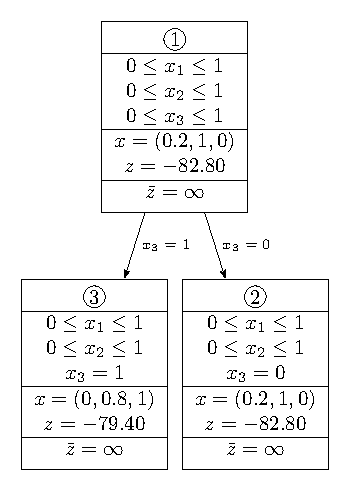
\includegraphics[width=.5\linewidth]{question/forest/1.pdf}
\end{figure}

Pour les lignes~\Circled{4} à \Circled{9}, il y a d’abord une contrainte sur $x_2$, puis sur $x_3$. Ce développement est représenté à la figure~\ref{arbre2}.

\begin{figure}[htbp]
	\caption{Branche $x_2$ puis $x_3$}
	\label{arbre2}
	\centering
	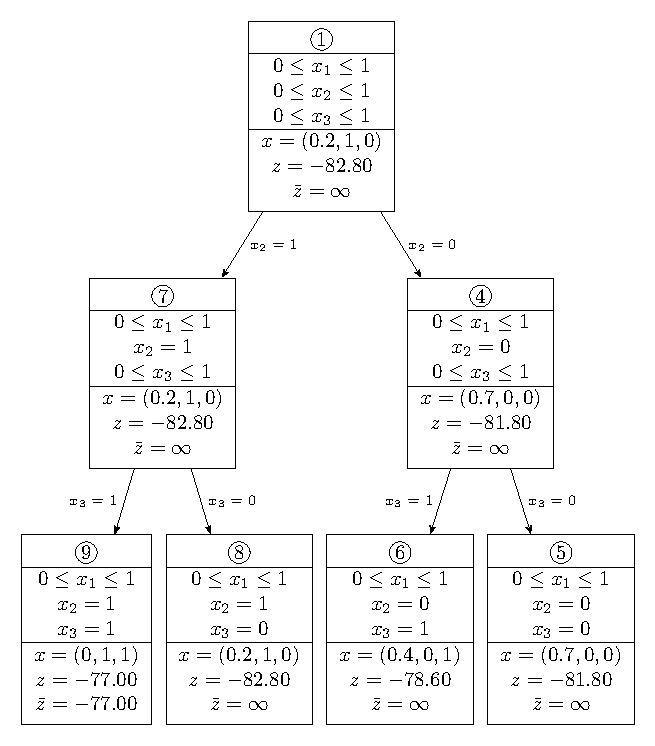
\includegraphics[width=.8\linewidth]{question/forest/2.pdf}
\end{figure}

Les lignes~\Circled{10} à \Circled{12} et \Circled{19} à \Circled{21} sont le résultat d’une contrainte sur $x_1$ puis sur $x_3$. Ce qui correspond à la figure~\ref{arbre3}.

\begin{figure}[htb]
	\caption{Branche $x_1$ puis $x_3$}
	\label{arbre3}
	\centering
	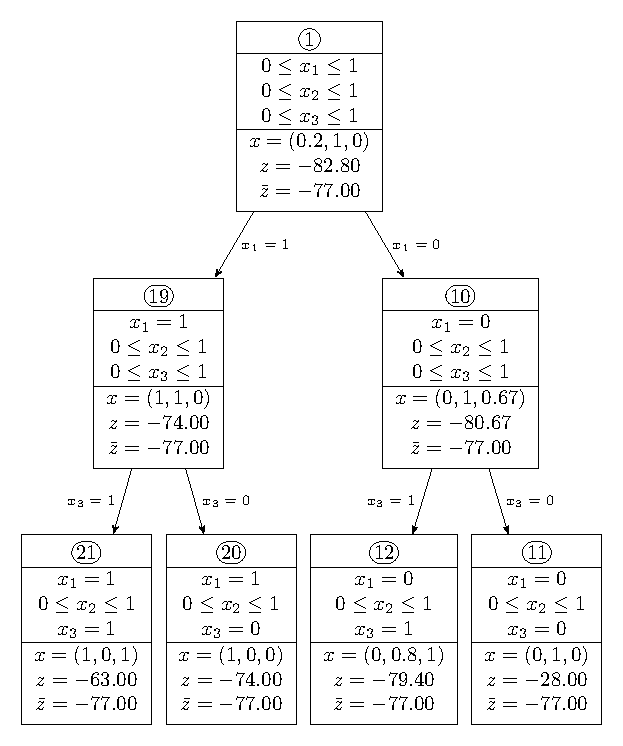
\includegraphics[width=.8\linewidth]{question/forest/3.pdf}
\end{figure}

Finalement, les lignes restantes sont le résultat d’une contrainte sur $x_1$, puis sur $x_2$ et $x_3$. Le graphe de cet arbre est représenté à la figure~\ref{arbre4}.

\begin{figure*}[htb]
	\caption{Branche $x_1$ puis $x_2$ et $x_3$}
	\label{arbre4}
	\centering
	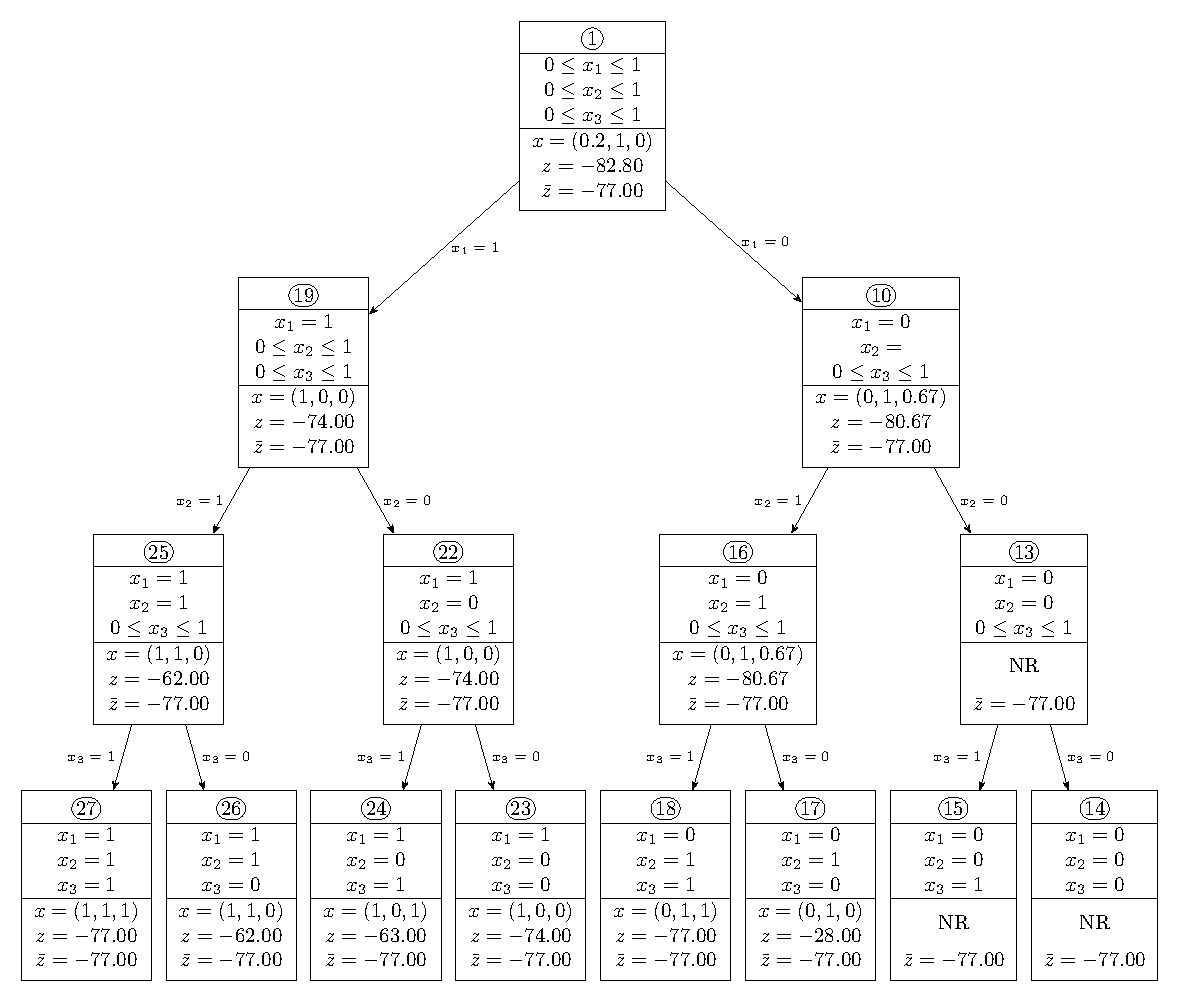
\includegraphics[width=.8\linewidth]{question/forest/4.pdf}
\end{figure*}
